\documentclass[10pt,a4paper]{article}
\usepackage[utf8]{inputenc}

\usepackage[landscape,margin=1cm]{geometry}
\usepackage[italian]{babel}


% colour themes to come. KnitR?

%-------------------------

\title{Cheatsheet Modelli di Calcolo e Algoritmi Avanzati}
\author{Paolo Speziali}
\date{Giugno 2022}
\usepackage[default]{raleway}
\usepackage{fontawesome}
\usepackage[T1]{fontenc}

\usepackage{hyperref}
\usepackage{enumitem}
\usepackage{lipsum}

\usepackage{xcolor}
\definecolor{customcolor}{HTML}{616AC5}
\definecolor{alert}{HTML}{CD5C5C}
\definecolor{w3schools}{HTML}{4CAF50}
\definecolor{subbox}{gray}{0.60}
\definecolor{codecolor}{HTML}{FFC300}
\colorlet{xx}{customcolor}


%--------------------------Editor mode.

\usepackage
[citestyle=authoryear,
sorting=nty,	  		%Sorts bibliography by year, name, title
autocite=footnote, 		%Autocite command generates footnotes
autolang=hyphen, 		
mincrossrefs=1, 	
backend=biber]
{biblatex}

\DeclareFieldFormat{postnote}{#1}
\DeclareFieldFormat{multipostnote}{#1}
\DeclareAutoCiteCommand{footnote}[f]{\footcite}{\footcites}

\bibliography{literature}
%----------------------------------------
%--------------------------------------------------------------------------------
\usepackage{tcolorbox}

\tcbuselibrary{most,listingsutf8,minted}

\tcbset{tcbox width=auto,left=1mm,top=1mm,bottom=1mm,
right=1mm,boxsep=1mm,middle=1pt}

\newenvironment{mycolorbox}[2]{%
\begin{tcolorbox}[grow to left by=-1em,grow to right by=-1em,capture=minipage,fonttitle=\large\bfseries, enhanced jigsaw,boxsep=1mm,colback=#1!30!white,on line,tcbox width=auto, toptitle=0mm,colframe=#1,opacityback=0.7,nobeforeafter,title=#2]%
}{\end{tcolorbox}\\[0.2em]}

\newenvironment{subbox}[2]{%
\begin{tcolorbox}[capture=minipage,fonttitle=\normalsize\bfseries, enhanced jigsaw,boxsep=1mm,colback=#1!30!white,on line,tcbox width=auto,left=0.3em,top=1mm, toptitle=0mm,colframe=#1,opacityback=0.7,nobeforeafter,title=#2]\footnotesize %
}{\normalsize\end{tcolorbox}\vspace{0.1em}}

\newenvironment{multibox}[1]{%
\begin{tcbraster}[raster columns=#1,raster equal height,nobeforeafter,raster column skip=1em,raster left skip=1em,raster right skip=1em]}{\end{tcbraster}}

\newenvironment{textbox}[1]{\begin{mycolorbox}{customcolor}{#1}}{\end{mycolorbox}}

%-------------------------------
\newtcblisting{codebox}[2]{colback=codecolor!5,colframe=codecolor!80!black,listing only, 
minted options={numbers=left,style=tcblatex,fontsize=\tiny,breaklines,autogobble,linenos,numbersep=3mm},
left=5mm,enhanced,
title=#2, fonttitle=\bfseries,
listing engine=minted,minted language=#1}

%--------------------------------------------------------------------------------
\newcommand{\punkti}{~\lbrack\dots\rbrack~}

\renewenvironment{quote}
               {\list{\faQuoteLeft\phantom{ }}{\rightmargin\leftmargin}%
                \item\relax\scriptsize\ignorespaces}
               {\unskip\unskip\phantom{xx}\faQuoteRight\endlist}
               

%--------------------------------------------------------------------------------
\newcommand{\bgupper}[3]{\colorbox{#1}{\color{#2}\huge\bfseries\MakeUppercase{#3}}}
\newcommand{\bg}[3]{\colorbox{#1}{\bfseries\color{#2}#3}}

\newcommand{\mycommand}[2]{{\ttfamily\detokenize{#1}}~\dotfill{}~{\footnotesize #2}\\}
\newcommand{\sep}{{\scriptsize~\faCircle{ }~}}


\newcommand{\bggreen}[1]{\medskip\bgupper{w3schools}{black}{#1}\\[0.5em]}
\newcommand{\green}[1]{\smallskip\bg{w3schools}{white}{#1}\\}
\newcommand{\red}[1]{\smallskip\bg{alert}{white}{#1}\\}

\usepackage{multicol}
\setlength{\columnsep}{30pt}

\setlength{\parindent}{0pt}
\pagestyle{empty}

\usepackage{csquotes}

\newcommand{\loremipsum}{Lorem ipsum dolor sit amet.}

\tolerance=1
\emergencystretch=\maxdimen
\hyphenpenalty=10000
\hbadness=10000


%--------------------------------------------------------------------------------
\begin{document}
\small
\begin{multicols}{3}

\maketitle
\thispagestyle{empty}


\section{Linguaggi e grammatiche}


\begin{textbox}{Tipi di grammatiche}

\red{Tipo 0}
Detta anche \textbf{non limitata}, ammette \textbf{qualunque tipo}
di produzione, anche quelle che accorciano le forme di
frase, come ad esempio quelle che si ottengono da \(\varepsilon\)-produzioni
(es. \(aA\,\rightarrow\,b\,|\,\varepsilon\)).

\red{Tipo 1}
Detta anche \textbf{context-sensitive}, ammette \textbf{qualunque tipo}
di produzione che \textbf{non accorci} le forme di frase
(es. \(aA\,\rightarrow\,Bb\)).

\red{Tipo 2}
Detta anche \textbf{context-free}, ammette produzioni in cui
il termine sinistro è formato da un solo non terminale
e la forma di frase non si accorcia mai \\
(es. \(A\,\rightarrow\,aBb\)).

\red{Tipo 3}
Detta anche \textbf{regolare}, ammette produzioni in cui
il termine sinistro è formato da un solo non terminale
e il termine destro o da un solo terminale o da un
terminale seguito da un non terminale\\
(es. \(aA\,\rightarrow\,b\,|\,aB\)).

\end{textbox}


\begin{textbox}{Pumping Lemma per L. Regolari}
Se L è un linguaggio regolare allora \\
\(\exists \, n \, > \, 0\) tale che \(\forall \, z \, \in \, L \) e
\(|z| \, \geq \, n\),\\si ha che
\(\exists \, u \, ,v \, ,w\) tali che:
\begin{enumerate}[leftmargin=*]
    \item \(z\, =\, uvw\)
    \item \(|uv|\, \leq\,  n\)
    \item \(|v|\, \geq\,  1\)
    \item \(uv^iw\,\in\,L,\,\forall\,i\,\geq\,0\)
\end{enumerate}

\end{textbox}

\begin{textbox}{Da Gram. Reg. a Esp. Reg.}
Dal sistema di equazioni lineari si ricava una espressione regolare
applicando le due tecniche seguenti ripetutamente:
\begin{itemize}[leftmargin=*]
    \item \textbf{Sostituzione}: si può sostituire un simbolo non terminale con una espressione equivalente \\
    (es. \(A\, aB\, +\, b,\, B\, =\, cA\,\Rightarrow \,  =\, acA\, +\, b)\)
    \item \textbf{Eliminazione della ricorsione}: si può sostituire la prima equazione con la seconda\\
    \(A\,=\,\alpha_1A\,+\,\alpha_2A\,+\,...\,+\
    \alpha_nA\,+\,\beta_1\,+\,\beta_2\,+\,...\,+\
    \beta_n\) \\
    \(A\,=\,(\alpha_1\,+\,\alpha_2\,+\,...\,+\
    \alpha_n\,)^\ast(\beta_1\,+\,\beta_2\,+\,...\,+\
    \beta_n)\)
\end{itemize}

\end{textbox}


\begin{textbox}{Myhill-Nerode}
\lipsum[1]

\end{textbox}

\begin{textbox}{Forma ridotta}
Una grammatica G CF è in forma ridotta se:
\begin{itemize}[leftmargin=*]
    \item G non contiene \(\varepsilon\)-produzioni
    se non sull’assioma, ed in tal caso l’assioma non
    compare a destra di nessuna produzione;
    \item G non contiene simboli inutili, cioè non fecondi o non generabili;
    \item G non contiene produzioni unitarie\\(cioè del tipo \(A\,\rightarrow\,B\)).
\end{itemize}

\end{textbox}

\begin{textbox}{Forma normale di Chomsky (CNF)}
Una grammatica G CF è in CNF se tutte le sue produzioni sono del tipo \(A\,\rightarrow\,BC\) o \(A\,\rightarrow\,a\).\\
Per arrivarci si porta G in forma ridotta e si sostituisce ogni terminale \(a\) con un non terminale \(X_a\) in tutte le produzioni
in cui compare \(a\) ed si introduce la produzione \(X_a\,\rightarrow\,a\)
(la forma ottenuta a questo punto si chiama \textbf{quasi CFN}).\\
Infine si sotituisce ricorsivamente ogni produzione del tipo:\\
\(A\,\rightarrow\,BC\alpha\) con le seguenti:
\(A\,\rightarrow\,BD\), \(D\,\rightarrow\,C\alpha\) dove D è un nuovo non terminale.
\end{textbox}


\begin{textbox}{Forma normale di Greibach (GNF)}
Una grammatica G CF è in GNF se tutte le sue produzioni sono del tipo \(A\,\rightarrow\,a\beta\), dove \(\beta\) è una sequenza (eventualmente vuota) di non terminali e \(a\)  è un simbolo terminale.\\
\end{textbox}

\begin{textbox}{Pumping Lemma per L CF}
Se L è un linguaggio CF allora \\
\(\exists \, n \, > \, 0\) tale che \(\forall \, z \, \in \, L \) e
\(|z| \, \geq \, n\),\\si ha che
\(\exists \, u \, ,v \, ,w \, ,x \, ,y\) tali che:
\begin{enumerate}[leftmargin=*]
    \item \(z\, =\, uvwxy\)
    \item \(|vwx|\, \leq\,  n\)
    \item \(|vx|\, \geq\,  1\)
    \item \(uv^iwx^iy\,\in\,L,\,\forall\,i\,\geq\,0\)
\end{enumerate}
\end{textbox}


%--------------------------------------------------------------
\section{Macchine di Turing}



\begin{textbox}{Lorem Ipsum}
test  \sep test \sep test \sep test

\bigskip

\green{Visualize}
\begin{enumerate}
\item \textbf{present} your data
\item \textbf{analyze} the information
\item \textbf{explore} the findings
\end{enumerate}

\end{textbox}


\begin{textbox}{Voyant Tools}
 \href{https://voyant-tools.org/}{Voyant Tools} \sep \href{https://voyant-tools.org/}{Voyant Tools}

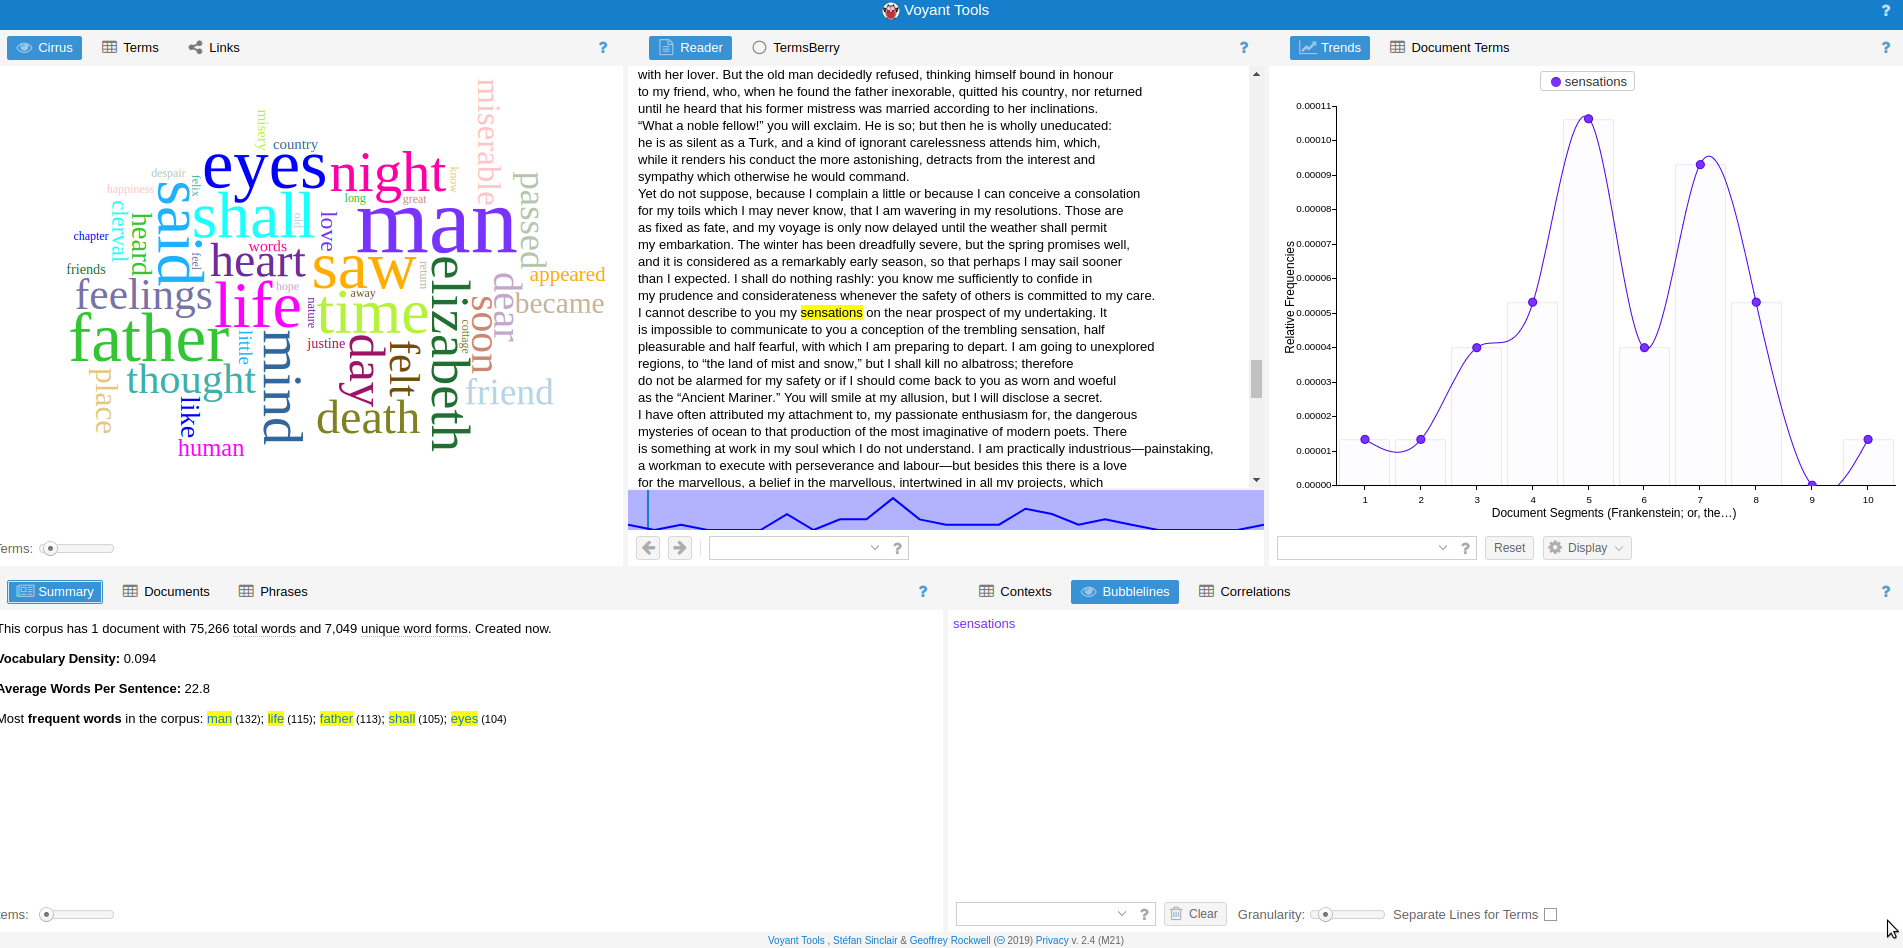
\includegraphics[width=\textwidth]{voyant.png}
\end{textbox}




\begin{textbox}{Project Gutenberg Texts}
\begin{tabular}{r|p{0.8\textwidth}}\scriptsize
    84 & \href{http://www.gutenberg.org/ebooks/84}{Frankenstein; Or, The Modern Prometheus by Mary Wollstonecraft Shelley} \\
    6087 & \href{https://www.gutenberg.org/ebooks/6087}{The Vampyre; a Tale by John William Polidori} \\
    696 & \href{https://www.gutenberg.org/ebooks/696}{The Castle of Otranto by Horace Walpole} \\
    42 & \href{https://www.gutenberg.org/ebooks/42}{The Strange Case of Dr. Jekyll and Mr. Hyde by Robert Louis Stevenson}
\end{tabular}

\end{textbox}





\begin{textbox}{Key concepts}
\red{Bag-of-words (BOW)}


\green{\emph{Zipf's Law}}

\mycommand{_&§!$§/()$}{code}
\mycommand{shutdown -h now}{to shutdown}

\end{textbox}


%--------------------------------------------------------------
\section{Programming}

\subsection{Code boxes}


% first argument: minted programming language name, for example.. css, c, cpp, etc.
\begin{codebox}{r}{Code box using R}
# Install
install.packages("tm")  # for text mining

# Load
library("tm")

# text <- readLines(file.choose())
# Read the text file from internet
filePath <- "http://www.internet.com/text.txt"
text <- readLines(filePath)

\end{codebox}


% first argument: minted programming language name, for example.. css, c, cpp, etc.
\begin{codebox}{cpp}{Code box using C++}
for (auto element : vector) 
{
    sum += element;
}
\end{codebox}

\newpage
\section{Smaller Subboxes}
\subsection{Subboxes}
%---------------------------------------------
\begin{multibox}{2} % number of boxes in a row
\begin{subbox}{subbox}{test}
\tiny


\bg{alert}{white}{test} 
\bggreen{test}\\

\end{subbox}
\begin{subbox}{customcolor}{test}
\scriptsize


\bgupper{w3schools}{black}{test}\\
\tiny
tiny font

\mycommand{$\lxor$}{XOR}
\mycommand{$\lor$}{OR}
\end{subbox}
\end{multibox}




%---------------------------------------------
\begin{multibox}{2} % number of boxes in a row
\begin{subbox}{subbox}{ Infos}

\bg{alert}{white}{bla}\\
\bgupper{w3schools}{black}{XX}\\

\end{subbox}
\begin{subbox}{customcolor}{ Infos}

\end{subbox}
\end{multibox}


\begin{textbox}{Subboxes}
%---------------------------------------------
\begin{multibox}{2} % number of boxes in a row
\begin{subbox}{subbox}{test}

\red{test} 
\bggreen{test}
\href{https://latex-ninja.com}{Link}
\end{subbox}
\begin{subbox}{customcolor}{test}
\scriptsize


\bggreen{test}
\tiny
super small font

\mycommand{$\land$}{AND $\land$}
\mycommand{$\lor$}{OR $\lor$}
\end{subbox}
\end{multibox}

%---------------------------------------------
\begin{multibox}{2} % number of boxes in a row
\begin{subbox}{subbox}{ Info}

\red{bla}\\
\bggreen{XX}\\

\end{subbox}
\begin{subbox}{customcolor}{Info}

\end{subbox}
\end{multibox}
\end{textbox}


%--------------------------------------------------------------

\begin{textbox}{bla}


\bgupper{w3schools}{black}{test}\\
\bg{alert}{white}{bla}
\begin{enumerate}
    \item \emph{bla}: bla.
    \item bla.
\end{enumerate}

%---------------------------------------------
\begin{multibox}{3} % number of boxes in a row
\begin{subbox}{subbox}{test}
info
\end{subbox}
\begin{subbox}{customcolor}{test}
$p \to q$
\mycommand{CTRL+C}{copy}
\end{subbox}
\begin{subbox}{subbox}{ Infos}
bla \\
more text
\end{subbox}
\end{multibox}

%---------------------------------------------
\begin{multibox}{3} % number of boxes in a row
\begin{subbox}{subbox}{ Infos}
info
\end{subbox}
\begin{subbox}{customcolor}{ Infos}
$p \to q$
\end{subbox}
\begin{subbox}{subbox}{ Infos}
bla \\
more text
\end{subbox}
\end{multibox}

\end{textbox}


%---------------------------------------------
\AtNextBibliography{\footnotesize}
\printbibliography  
\end{multicols}

\end{document}
